%%%% proposta_pt.tex
%%%% Project specification paper based on the IJCAI--ECAI 26 template.

\typeout{Project paper using IJCAI--ECAI 26 formatting}

\documentclass{article}
\pdfpagewidth=8.5in
\pdfpageheight=11in

% Official IJCAI--ECAI 26 style file.
% Compile from this directory so the relative path resolves correctly.
\usepackage{../FormattingGuidelines-IJCAI-ECAI-26/ijcai26}

% Packages required/recommended by the official template.
\usepackage{times}
\usepackage{soul}
\usepackage{url}
\usepackage[hidelinks]{hyperref}
\usepackage[utf8]{inputenc}
\usepackage[small]{caption}
\usepackage{graphicx}
\usepackage{tikz}
\usetikzlibrary{positioning,arrows.meta}
\usepackage{amsmath}
\usepackage{amsthm}
\usepackage{booktabs}
\usepackage{algorithm}
\usepackage{algorithmic}
\usepackage[switch]{lineno}

% Keep line numbers enabled for a submission. Disable for camera-ready.
\linenumbers

\urlstyle{same}

% Optional theorem environments.
\newtheorem{example}{Example}
\newtheorem{theorem}{Theorem}

% Required PDF metadata block. Keep unchanged.
\pdfinfo{
/TemplateVersion (IJCAI.2026.0)
}

\title{Segmenta\c{c}\~ao sem\^antica de trajet\'orias AIS para dete\c{c}\~ao de atividade de pesca usando janelas sobrepostas e p\'os-processamento temporal}

% For an anonymous submission, replace this block with the track-approved
% anonymous author declaration. For the camera-ready version, provide all
% author and affiliation information.
\author{
    Dinis Soveral Botelho Rosa
    \affiliations
    University of Coimbra / Department of Informatics Engineering
    \emails
    dinisrosa22@gmail.com
}

\begin{document}

\maketitle

\begin{abstract}
A pesca ilegal, n\~ao declarada e n\~ao regulamentada (IUU) \'e uma das maiores
amea\c{c}as \`a sustentabilidade dos oceanos. O \emph{Automatic Identification
System} (AIS) permite monitorizar a atividade dos navios \`a escala global, mas
transformar trajet\'orias AIS em dete\c{c}\~oes \'uteis para a fiscaliza\c{c}\~ao
exige m\'etodos robustos e interpret\'aveis. Propomos investigar se a combina\c{c}\~ao de janelas sobrepostas e
p\'os-processamento temporal melhora a qualidade e a estabilidade da segmenta\c{c}\~ao
sem\^antica de trajet\'orias AIS para detetar atividade de pesca, como apoio \`a
decis\~ao de inspetores humanos (\emph{human-in-the-loop}). O sistema segue princ\'ipios
da Intelig\^encia Artificial Centrada no Humano (HCAI), incorporando explicabilidade,
confian\c{c}a calibrada e decis\~ao humana final.
A abordagem ser\'a avaliada sobre um conjunto p\'ublico de 128 trajet\'orias de pesca
anotadas (Kaggle), comparando com \emph{baselines} como um \emph{Hidden Markov Model} e
a segmenta\c{c}\~ao sem\^antica de Wu et al.~\cite{wu2022}, atrav\'es de m\'etricas como
precis\~ao, sensibilidade, F1 e \emph{intersection-over-union}, complementadas por
an\'alise qualitativa.
\end{abstract}

\section{Problema e Motiva\c{c}\~ao}
\label{sec:problema-motivacao}

A pesca ilegal, n\~ao declarada e n\~ao regulamentada (IUU) \'e uma das principais
amea\c{c}as \`a sustentabilidade dos oceanos: estima-se que represente at\'e cerca de
20\% da captura mundial de pescado~\cite{agnew2009}, com perdas econ\'omicas na ordem das dezenas de
milhares de milh\~oes de d\'olares por ano, al\'em de agravar a sobre-explora\c{c}\~ao
dos \emph{stocks}, degradar habitats e estar associada a condi\c{c}\~oes de trabalho
ilegais~\cite{chuaysi2020}. Combater este fen\'omeno exige saber onde, quando e quais os
navios que est\~ao efetivamente a pescar --- uma tarefa imposs\'ivel de realizar apenas
por inspe\c{c}\~ao humana, dada a escala da frota mundial e o volume de dados de
tr\'afego mar\'itimo.

O AIS transmite, em intervalos de poucos segundos, a posi\c{c}\~ao, o rumo e a
velocidade de cada navio, tornando-se a principal fonte de dados para monitorizar a
atividade piscat\'oria \`a escala global~\cite{natale2015,kroodsma2018}. A partir destas
trajet\'orias \'e poss\'ivel inferir os padr\~oes de movimento caracter\'isticos da
pesca --- velocidades reduzidas, mudan\c{c}as de rumo frequentes e deslocamentos em
ziguezague --- distinguindo-os dos da navega\c{c}\~ao em tr\^ansito. O problema que este
projeto aborda \'e, assim, o de \textbf{classificar automaticamente, ao longo de uma
trajet\'oria AIS, os intervalos temporais correspondentes a atividade de pesca versus
navega\c{c}\~ao}, de forma robusta e interpret\'avel.

A motiva\c{c}\~ao \'e dupla. Por um lado, t\'ecnica: os modelos atuais de
segmenta\c{c}\~ao de trajet\'orias tendem a produzir segmenta\c{c}\~oes ruidosas e
sens\'iveis a pequenas perturba\c{c}\~oes, que podem ganhar consist\^encia com janelas
sobrepostas e p\'os-processamento temporal. Por outro, humana: este sistema destina-se a apoiar
agentes de fiscaliza\c{c}\~ao e autoridades de gest\~ao das pescas, pelo que deve ser
\textbf{fi\'avel, explic\'avel e concebido para coopera\c{c}\~ao humano-IA} ---
apresentando as suas decis\~oes de forma transparente e deixando a decis\~ao final a um
inspetor humano. O projeto enquadra-se assim na \'area da Intelig\^encia Artificial
Centrada no Humano (HCAI), em particular nos t\'opicos da coopera\c{c}\~ao humano-IA e da
IA fi\'avel e respons\'avel.

\section{Contexto}
\label{sec:contexto}

Os primeiros trabalhos de identifica\c{c}\~ao autom\'atica de atividade de pesca
basearam-se em m\'etodos probabil\'isticos sobre dados de \emph{Vessel Monitoring
System} (VMS). Peel e Good~\cite{peel2011} e Vermard et al.~\cite{vermard2010}
propuseram \emph{hidden Markov models} (HMM) para distinguir estados de pesca e de
navega\c{c}\~ao a partir de s\'eries temporais de posi\c{c}\~oes. A ado\c{c}\~ao
generalizada do AIS alargou a escala desta monitoriza\c{c}\~ao. Natale et
al.~\cite{natale2015} mapearam o esfor\c{c}o de pesca europeu a partir de AIS, e
Kroodsma et al.~\cite{kroodsma2018} constru\'iram um mapa global da pegada da pesca
comercial.

Mais recentemente, a segmenta\c{c}\~ao sem\^antica de trajet\'orias emergiu como
formalismo adequado ao problema: em vez de classificar pontos isolados, divide-se a
trajet\'oria em segmentos homog\'eneos dotados de significado. Soares J\'unior et
al.~\cite{soares2018} propuseram uma abordagem semi-supervisionada baseada no princ\'ipio
\emph{Minimum Description Length}, e Wu et al.~\cite{wu2022} aplicaram a
segmenta\c{c}\~ao sem\^antica a trajet\'orias AIS para detetar atividades de pesca
completas --- a refer\^encia central deste projeto. Em paralelo, os m\'etodos de
aprendizagem profunda t\^em vindo a dominar a \'area: redes com aten\c{c}\~ao para a
classifica\c{c}\~ao de navios~\cite{cheng2025}, aprendizagem espa\c{c}o-temporal
local-global (FishFormer)~\cite{wang2026}, campos de Gram (\emph{Gramian Angular
Field}) para reconhecimento de padr\~oes~\cite{hu2026} e m\'etodos geom\'etricos
semi-supervisionados~\cite{ferreira2022}. Complementarmente, a literatura cobre a
identifica\c{c}\~ao de comportamento e a rastreabilidade no combate \`a pesca
IUU~\cite{chuaysi2020}, a dete\c{c}\~ao de atividade em dados AIS
longitudinais~\cite{arasteh2020}, a classifica\c{c}\~ao de
trajet\'orias~\cite{luo2023,xing2023} e compara\c{c}\~oes sistem\'aticas de m\'etodos
sobre VMS~\cite{guillot2018,ghazizadeh2019}.
 No que respeita \`a dimens\~ao humana, a IA Centrada no Humano (HCAI)~\cite{shneiderman2020}
 defende sistemas fi\'aveis e explic\'aveis que apoiem a decis\~ao humana em vez de a
 substitu\'irem.

Apesar destes avan\c{c}os, subsistem limita\c{c}\~oes que motivam o projeto. Em primeiro
lugar, as predi\c{c}\~oes ponto-a-ponto tendem a ser ruidosas e a produzir fronteiras de
segmento inst\'aveis. Este projeto prop\~oe combinar janelas sobrepostas com
p\'os-processamento temporal para suavizar e estabilizar essas fronteiras, e avaliar
explicitamente o efeito dessa combina\c{c}\~ao na estabilidade dos segmentos. Em segundo
lugar, a dimens\~ao humana \'e frequentemente secundarizada: para uso real em
fiscaliza\c{c}\~ao, o sistema deve ser explic\'avel e cooperar com o inspetor, e n\~ao
atuar como uma ``caixa preta'' inquestion\'avel. Face a Wu et al.~\cite{wu2022}, que
detetam atividades de pesca completas por segmenta\c{c}\~ao sem\^antica, este projeto
acrescenta a avalia\c{c}\~ao da estabilidade temporal obtida com as janelas sobrepostas e
o p\'os-processamento, bem como a perspetiva de coopera\c{c}\~ao humano-IA. \'E nestas
duas dimens\~oes --- robustez temporal e centralidade humana --- que o projeto se
posiciona.

\section{Objetivos}
\label{sec:objetivos}

O objetivo principal \'e desenvolver um sistema de segmenta\c{c}\~ao sem\^antica de
trajet\'orias AIS que detete atividade de pesca de forma robusta e interpret\'avel,
combinando \textbf{janelas sobrepostas} e \textbf{p\'os-processamento temporal}, e
concebido como \textbf{apoio \`a decis\~ao de inspetores} (\emph{human-in-the-loop}).
Deste objetivo decorrem os seguintes objetivos espec\'ificos:

\begin{enumerate}
    \item Construir um \emph{pipeline} de pr\'e-processamento do conjunto de dados AIS
    (limpeza, normaliza\c{c}\~ao, engenharia de caracter\'isticas e janelamento com
    sobreposi\c{c}\~ao).
    \item Implementar e treinar um modelo de classifica\c{c}\~ao de janelas (por exemplo,
     redes recorrentes ou convolucionais com aten\c{c}\~ao), usando a segmenta\c{c}\~ao de
     Wu et al.~\cite{wu2022} e/ou um HMM~\cite{peel2011} como \emph{baselines}.
    \item Conceber e avaliar um p\'os-processamento temporal que combine as predi\c{c}\~oes
    das janelas sobrepostas e regularize as fronteiras dos segmentos.
    \item Avaliar o sistema quantitativamente (m\'etricas por segmento e por ponto) e
    qualitativamente (visualiza\c{c}\~ao e casos de estudo).
    \item Dotar o sistema de elementos de explicabilidade (por exemplo, atribui\c{c}\~oes de
    import\^ancia~\cite{lundberg2017} e confian\c{c}a calibrada~\cite{guo2017}) que sustentem a
    decis\~ao do inspetor.
\end{enumerate}

De forma mais precisa, o trabalho guia-se por tr\^es perguntas de investiga\c{c}\~ao:
(RQ1) em que medida as janelas sobrepostas reduzem a instabilidade das fronteiras da
segmenta\c{c}\~ao relativamente a janelas n\~ao sobrepostas? (RQ2) em que medida o
p\'os-processamento temporal reduz a fragmenta\c{c}\~ao e melhora a concord\^ancia entre
os segmentos previstos e os anotados? (RQ3) qual a intera\c{c}\~ao entre sobreposi\c{c}\~ao
e p\'os-processamento na qualidade e estabilidade da segmenta\c{c}\~ao?

Considera-se o trabalho bem-sucedido se (i) caracterizar quantitativamente o efeito das
janelas sobrepostas e do p\'os-processamento na qualidade e estabilidade da
segmenta\c{c}\~ao, procurando melhor\'a-las face aos \emph{baselines} --- aceitando como
resultado v\'alido a demonstra\c{c}\~ao de que uma componente n\~ao traz ganho ---, (ii)
produzir segmenta\c{c}\~oes temporalmente est\'aveis e (iii) fornecer justifica\c{c}\~oes
audit\'aveis que permitam a um inspetor humano validar as dete\c{c}\~oes. As contribui\c{c}\~oes esperadas s\~ao: um m\'etodo de janelas sobrepostas
com p\'os-processamento temporal para a dete\c{c}\~ao de pesca; uma avalia\c{c}\~ao que
integre a perspetiva HCAI (explicabilidade e coopera\c{c}\~ao humano-IA); e evid\^encia
emp\'irica sobre o valor do p\'os-processamento na robustez das dete\c{c}\~oes.

\section{Abordagem}
\label{sec:abordagem}

O sistema ser\'a organizado num \emph{pipeline} de cinco etapas (Figura~\ref{fig:pipeline}). (1)~\emph{Ingest\~ao e
pr\'e-processamento}: os dados do ficheiro CSV s\~ao importados, os \emph{outliers} e \emph{gaps} temporais s\~ao
tratados e as caracter\'isticas normalizadas; caracter\'isticas derivadas (como a acelera\c{c}\~ao) s\~ao calculadas a partir das
coordenadas e do tempo; a velocidade, o rumo, a varia\c{c}\~ao de rumo e a dist\^ancia \`a
costa j\'a v\^em no dataset e n\~ao s\~ao recalculados. (2)~\emph{Janelamento}: cada trajet\'oria \'e dividida em
janelas de comprimento fixo com sobreposi\c{c}\~ao, de modo a dar contexto local a cada
ponto e a mitigar os efeitos de fronteira. (3)~\emph{Classifica\c{c}\~ao}: cada janela \'e
classificada como pesca ou navega\c{c}\~ao por um modelo de aprendizagem profunda, cuja
arquitetura (recorrente ou convolucional, possivelmente com aten\c{c}\~ao) ser\'a selecionada
empiricamente no protocolo experimental, na linha de~\cite{cheng2025,wang2026}. (4)~\emph{P\'os-processamento temporal}: as
predi\c{c}\~oes das janelas sobrepostas s\~ao agregadas (por exemplo, por vota\c{c}\~ao
ponderada) e suavizadas com regulariza\c{c}\~ao temporal (por exemplo, uma suaviza\c{c}\~ao
via HMM ou vota\c{c}\~ao por vizinhan\c{c}a), produzindo segmentos cont\'iguos e
est\'aveis. (5)~\emph{Sa\'ida e explicabilidade}: o sistema devolve a trajet\'oria
segmentada com um n\'ivel de confian\c{c}a por segmento e justifica\c{c}\~oes
(import\^ancias de caracter\'isticas), apresentadas de forma a apoiar --- e n\~ao substituir
--- a decis\~ao do inspetor.

A implementa\c{c}\~ao utilizar\'a Python e o ecossistema PyTorch, scikit-learn e pandas,
num ambiente virtual dedicado. Como
\emph{baselines} ser\~ao usados um HMM~\cite{peel2011} e a segmenta\c{c}\~ao sem\^antica
de~\cite{wu2022}. As principais decis\~oes de desenho s\~ao: (i) janelas sobrepostas para
capturar contexto sem perder resolu\c{c}\~ao temporal; (ii) p\'os-processamento temporal para
garantir consist\^encia e estabilidade; e (iii) um canal de explicabilidade que torne cada
dete\c{c}\~ao audit\'avel por um humano.

\begin{figure}[t]
\centering
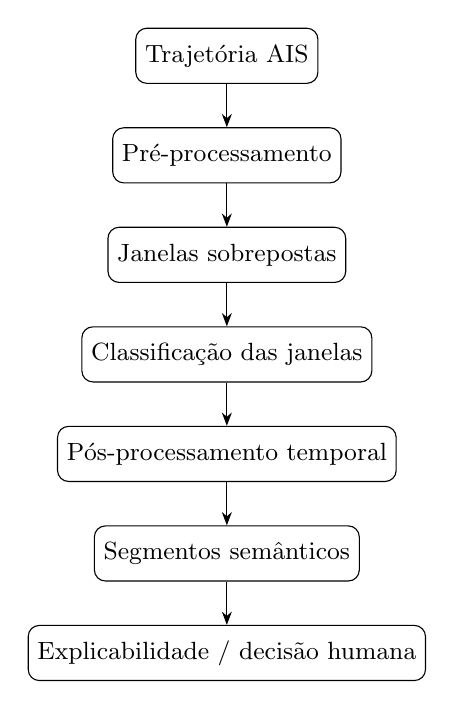
\begin{tikzpicture}[node distance=0.55cm, box/.style={draw, rounded corners, align=center, minimum height=0.7cm, font=\small}]
\node[box] (a) {Trajet\'oria AIS};
\node[box, below=of a] (b) {Pr\'e-processamento};
\node[box, below=of b] (c) {Janelas sobrepostas};
\node[box, below=of c] (d) {Classifica\c{c}\~ao das janelas};
\node[box, below=of d] (e) {P\'os-processamento temporal};
\node[box, below=of e] (f) {Segmentos sem\^anticos};
\node[box, below=of f] (g) {Explicabilidade / decis\~ao humana};
\draw[-{Stealth}] (a) -- (b);
\draw[-{Stealth}] (b) -- (c);
\draw[-{Stealth}] (c) -- (d);
\draw[-{Stealth}] (d) -- (e);
\draw[-{Stealth}] (e) -- (f);
\draw[-{Stealth}] (f) -- (g);
\end{tikzpicture}
\caption{Esquema do \emph{pipeline} proposto.}
\label{fig:pipeline}
\end{figure}

\section{Materiais e Dados}
\label{sec:materiais-dados}

Ser\'a usado o conjunto de dados p\'ublico \emph{Detailed Labelled Fishing Trajectories
from AIS} (Kaggle)~\cite{kaggleAIS}, que cont\'em 128 trajet\'orias de pesca anotadas, totalizando cerca de
1,03 milh\~oes de pontos. Cada ponto tem 13 atributos --- entre os quais o identificador do navio, o instante
temporal, a posi\c{c}\~ao (longitude e latitude), a velocidade, o rumo e a dist\^ancia \`a
costa --- e um r\'otulo. Os r\'otulos,
desequilibrados, distinguem cinco classes: pesca (\texttt{02-fishing},
\texttt{04-fishing}) e navega\c{c}\~ao (\texttt{01-sailing}, \texttt{03-sailing},
\texttt{05-sailing}). Como o objetivo \'e exclusivamente distinguir atividade de pesca de
navega\c{c}\~ao, as cinco classes s\~ao agregadas num problema bin\'ario (pesca vs.
navega\c{c}\~ao); o desequil\'ibrio natural entre as classes \'e mantido (sem reamostragem
nem pesos de classe), preservando as trajet\'orias completas.

As ferramentas incluem Python 3.14, o ambiente virtual do reposit\'orio, PyTorch,
scikit-learn, pandas e bibliotecas de visualiza\c{c}\~ao (matplotlib, geopandas). Quanto a
considera\c{c}\~oes \'eticas, os dados AIS s\~ao p\'ublicos, mas o uso do sistema em
fiscaliza\c{c}\~ao tem implica\c{c}\~oes que exigem cuidado: a dete\c{c}\~ao autom\'atica
n\~ao deve, por si s\'o, fundamentar san\c{c}\~oes (a decis\~ao humana \'e
obrigat\'oria); o sistema deve ser transparente e justo, evitando enviesamentos
sistem\'aticos contra determinados tipos de navio, regi\~oes ou comunidades de pesca; e a
confian\c{c}a deve ser calibrada para n\~ao induzir falsa seguran\c{c}a no inspetor.

\section{Avalia\c{c}\~ao}
\label{sec:avaliacao}

A avalia\c{c}\~ao ter\'a uma componente quantitativa e outra qualitativa.
Quantitativamente, o desempenho ser\'a medido por precis\~ao, sensibilidade (\emph{recall}),
F1 e \emph{intersection-over-union} (IoU) por segmento, comparando o sistema proposto com
os \emph{baselines} (HMM~\cite{peel2011} e Wu et al.~\cite{wu2022}). Para isolar a contribui\c{c}\~ao de cada
componente, ser\'a feito um estudo de abla\c{c}\~ao com quatro variantes: (i) sem
sobreposi\c{c}\~ao e sem p\'os-processamento; (ii) s\'o com sobreposi\c{c}\~ao; (iii) s\'o com
p\'os-processamento; e (iv) com sobreposi\c{c}\~ao e p\'os-processamento (m\'etodo proposto).
Ser\'a ainda analisada a robustez em fun\c{c}\~ao da taxa de sobreposi\c{c}\~ao (por exemplo,
0\%, 25\%, 50\% e 75\%) e do n\'ivel de regulariza\c{c}\~ao temporal. Al\'em das m\'etricas por
segmento e por ponto, medir-se-\'a a estabilidade da segmenta\c{c}\~ao atrav\'es da
fragmenta\c{c}\~ao (n\'umero de segmentos por trajet\'oria) e do erro de fronteira (desvio entre
o in\'icio/fim previsto e o real), entendendo por ``est\'avel'' uma segmenta\c{c}\~ao que muda
pouco sob pequenas altera\c{c}\~oes da janela ou do p\'os-processamento.

Os dados ser\~ao divididos de forma agrupada por navio em treino/valida\c{c}\~ao/teste
(70/15/15), garantindo que todas as trajet\'orias de um navio ficam no mesmo conjunto e
evitando fuga de informa\c{c}\~ao; os hiperpar\^ametros ser\~ao escolhidos apenas com treino
e valida\c{c}\~ao. Qualitativamente, ser\~ao produzidos mapas e gr\'aficos das trajet\'orias
com os segmentos preditos sobrepostos \`a verdade de refer\^encia, e analisados casos de
estudo de sucesso e de falha. Para a dimens\~ao HCAI, avaliar-se-\'a, de forma preliminar, a
explicabilidade das dete\c{c}\~oes (por exemplo, verificando se as atribui\c{c}\~oes de
import\^ancia~\cite{lundberg2017} correspondem aos padr\~oes de movimento esperados) e a
utilidade do sistema como apoio \`a decis\~ao, atrav\'es de uma prova de conceito visual
(\emph{dashboard}) que apresente a segmenta\c{c}\~ao, a confian\c{c}a por segmento e as
justifica\c{c}\~oes a um inspetor. O sistema segue princ\'ipios de IA centrada no
humano~\cite{shneiderman2020}, com confian\c{c}a calibrada~\cite{guo2017} e decis\~ao humana
final. Os resultados esperados incluem tabelas de m\'etricas, matrizes de confus\~ao, curvas
de robustez em fun\c{c}\~ao da sobreposi\c{c}\~ao e do p\'os-processamento, e
visualiza\c{c}\~oes de trajet\'orias.

% References may use the provided IJCAI named bibliography style.
\bibliographystyle{../FormattingGuidelines-IJCAI-ECAI-26/named}
\bibliography{references}

\end{document}